\documentclass[12pt, letterpaper] {article}

\parindent=5mm
\usepackage[spanish]{babel}

\usepackage{amssymb}
\usepackage{amsmath} 
\usepackage{amsfonts}

\usepackage[numbers,sort&compress]{natbib}
\usepackage{graphicx}

\usepackage{url}
\usepackage{hyperref}

\usepackage[top=25mm, bottom=20mm, left=1.5cm, right=1.5cm]{geometry}
\setlength{\parskip}{2mm}
\setlength{\parindent}{1pt}

\usepackage{listings}

\usepackage{float}

\usepackage[utf8]{inputenc}
\usepackage{graphicx} 
\usepackage{subfigure} 

\usepackage{color}
\usepackage{multirow}

\definecolor{dkgreen}{rgb}{0,0.6,0}
\definecolor{gray}{rgb}{0.5,0.5,0.5}
\definecolor{mauve}{rgb}{0.58,0,0.82}

\usepackage{color}
\usepackage{listings}
\lstset{ %
  language=R,                     % the language of the code
  basicstyle=\footnotesize,       % the size of the fonts that are used for the code
  numbers=left,                   % where to put the line-numbers
  numberstyle=\tiny\color{gray},  % the style that is used for the line-numbers
  stepnumber=1,                   % the step between two line-numbers. If it's 1, each line
                                  % will be numbered
  numbersep=5pt,                  % how far the line-numbers are from the code
  backgroundcolor=\color{white},  % choose the background color. You must add \usepackage{color}
  showspaces=false,               % show spaces adding particular underscores
  showstringspaces=false,         % underline spaces within strings
  showtabs=false,                 % show tabs within strings adding particular underscores
  frame=single,                   % adds a frame around the code
  rulecolor=\color{black},        % if not set, the frame-color may be changed on line-breaks within not-black text (e.g. commens (green here))
  tabsize=2,                      % sets default tabsize to 2 spaces
  captionpos=b,                   % sets the caption-position to bottom
  breaklines=true,                % sets automatic line breaking
  breakatwhitespace=false,        % sets if automatic breaks should only happen at whitespace
  title=\lstname,                 % show the filename of files included with \lstinputlisting;
                                  % also try caption instead of title
  keywordstyle=\color{blue},      % keyword style
  commentstyle=\color{dkgreen},   % comment style
  stringstyle=\color{mauve},      % string literal style
  escapeinside={\%*}{*)},         % if you want to add a comment within your code
  morekeywords={*,...}            % if you want to add more keywords to the set
} 

\usepackage{booktabs}
\usepackage[table,xcdraw]{xcolor}


\author{Ricardo Rosas Macías}

\title{Práctica 3: teoría de colas}

\date{\today}

\begin{document}

\maketitle



\section{Introducción}

La teoría de colas o líneas de espera, es un análisis matemático que permite estudiar el comportamiento sistemático de un procedimiento que tiene la capacidad de procesar muchos datos o tareas, sin aletargamiento que arruine la obtención de los parámetros de interés. 

 \section{Objetivo}

En la práctica se busca examinar el arreglo de las tareas del experimento, obtener los tiempos que tardan en realizarse y su duración al ejecutarse con un número de núcleos determinado. 

 \subsection{Descripción}

Lo que se debe hacer es \cite{elisawebTC}:
\begin{quotation}
 ``Examinar cómo las diferencias en los tiempos de ejecución de los diferentes ordenamientos cambian cuando se varía el número de núcleos asignados al cluster, utilizando como datos de entrada un vector que contiene primos grandes; descargados de \url{https://primes.utm.edu/lists/small/millions/} y no-primos con un mismo número de dígitos. Investiga también el efecto de la proporción de primos y no primos en el vector igual como la magnitud de los números incluidos en el vector con pruebas estadísticas adecuadas.''
\end{quotation}


\section{Resultados y conclusiones}

En términos generales para la lograr con el objetivo, se realizaron cambios en el código \cite{MPP3C}\cite{P3LSa} de tal forma que proporcione el comportamiento que tiene la ejecución del experimento con la proporción de primos y no primos. 

\begin{lstlisting}[language=R]
pd <- read.csv("primes1.txt", sep="", header = FALSE) #Primos descargados
pd$V1 <- NULL
pd$V10 <- NULL
pdm <- as.matrix(pd)
primos <- as.vector(t(pdm)) 

hastA<-20011
desde<-5381
hasta<-11827
replicas<-30
primo <- function(n) {
  for (i in 2:(n-1)) {
    if ((n > i && n %% i) == 0) { # residuo es cero
      return(FALSE)
    }
  }
  return(n)
}
primos <- numeric() # un vector vacio
for (n in desde:hastA) {
  primos <- c(primos, primo(n)) # combinar vectores
}

noprimo <- function(n) {
  for (i in 2:(n-1)) {
    if ((n > i && n %% i) == 0) { # residuo es cero
      return(n)
    }
  }
  return(FALSE)
}
noprimos <- numeric() # un vector vacio
for (m in desde:hasta) {
  noprimos <- c(noprimos, noprimo(m)) # combinar vectores
}

PC<-primos[which(primos>0)] # Primos crecientes 
NPC<-noprimos[which(noprimos>0)] # No primos crecientes
PD<- sort(a,decreasing = TRUE) # Primos decrecientes 
NPD<-sort(l,decreasing = TRUE) # No primos decrecientes
PA<-sample(a) # Primos aleatorios
NPA<-sample(d) # No primos aleatorios

e <- sample(a, size=420 ,replace = TRUE, prob = NULL)
f<-sample(l,size=420, replace = TRUE,prob=NULL)

primx <- function(n) {
  if (n == 1 || n == 2) {
    return(TRUE)
  }
  if (n %% 2 == 0) {
    return(FALSE)
  }
  for (i in seq(3, max(3, ceiling(sqrt(n))), 2)) {
    if ((n %% i) == 0) {
      return(FALSE)
    }
  }
  return(TRUE)
}

suppressMessages(library(doParallel))
registerDoParallel(makeCluster(detectCores()-2))
PCt <- numeric()
PDt <-numeric()
PAt <- numeric()
NPDt <-numeric()
NPCt <-numeric()
NPAt <-numeric()

for (r in 1:replicas) {
  PCt <- c(at, system.time(foreach(n = a, .combine=c) %dopar% primx(n))[3])
  PDt <- c(bt, system.time(foreach(n = b, .combine=c) %dopar% primx(n))[3])
  PAt <- c(vt, system.time(foreach(n = v, .combine=c) %dopar% primx(n))[3])
  NPDt <- c(dt, system.time(foreach(n = d, .combine=c) %dopar% primx(n))[3])
  NPCt <- c(lt, system.time(foreach(n = l, .combine=c) %dopar% primx(n))[3])   
  NPAt <- c(wt, system.time(foreach(n = w, .combine=c) %dopar% primx(n))[3]) 
  }
stopImplicitCluster()

mean(PCt)
mean(PDt)
mean(NPDt)
mean(NPCt)
mean(PAt)
mean(NPAt)
nucleos <- rep(1,20)
nucleos<-c(nucleos,rep(2,20))
digitos<-rep(5,10)
digitos<-c(digitos,rep(4,10))
digitos<-c(digitos,rep(3,10))
digitos<-c(digitos,rep(2,10))
digitos<-c(digitos,rep(1,10))
proportion<- rep(1,3)
proportion<-c(proportion,rep(2,3))
proportion<-c(proportion,rep(3,3))          
p<-c(1, 2, 3)
ordenamiento<-rep(p, 20)
\end{lstlisting}

Se realizaron gráficos de la simulación como se muestra en la figura \ref{Rfin}, en donde se puede observar en la figura \ref{Nu} el cambio de núcleos para realizar las tareas es ligeramente significativo, la media de tiempo promedio sube un poco pero permanece debajo del segundo cuartil. En cuanto el orden, en la figura \ref{Ord} se muestra que se tarda menos en analizar los datos de manera ascendente; como aparecen en el documento de texto que se descargo de la página web. Sin embargo, en la figura \ref{Pro} muestra una proporción, donde hay algunos cambios en la matriz respecto al tiempo del ciclo. Finalmente podemos observar en la figura \ref{Dig} el número de dígitos en el cual se distingue claramente que se tarda mucho más al realizar el análisis de números de 2 dígitos.

\begin{figure}[H]
\centering
\subfigure[Núcleos]{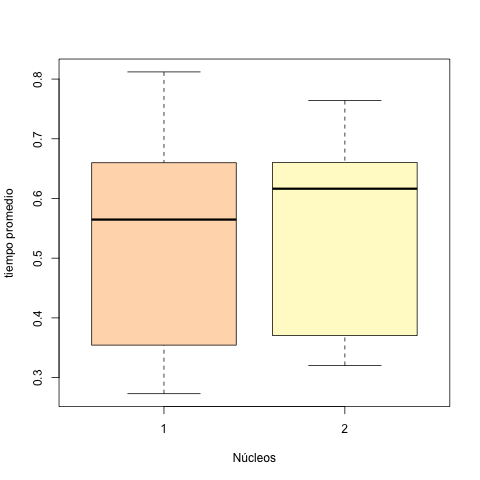
\includegraphics[width=80mm]{./nucleos} \label{Nu}}\vspace{-4mm}
\subfigure[Orden]{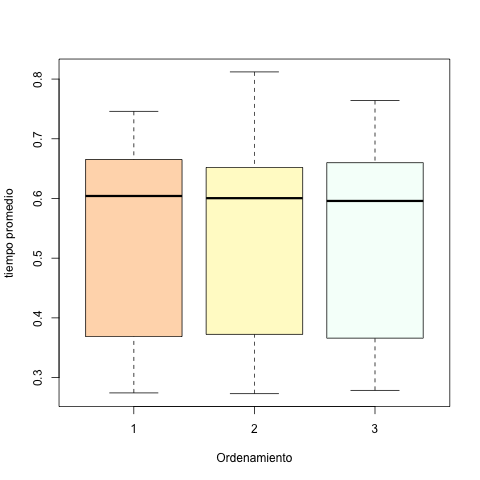
\includegraphics[width=80mm]{./ordenamiento} \label{Ord}}\vspace{-4mm}
\subfigure[Proporción]{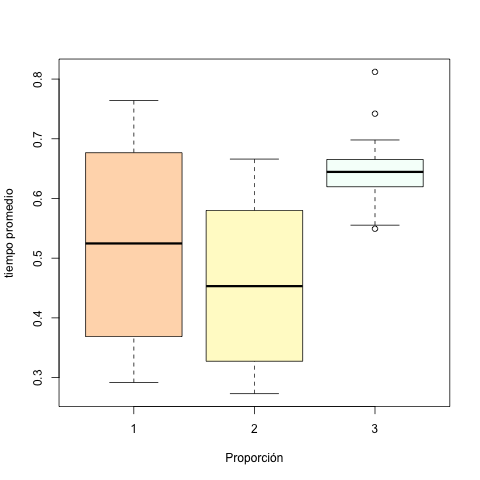
\includegraphics[width=80mm]{./proporcion} \label{Pro}}\vspace{-1mm}
\subfigure[Dígitos]{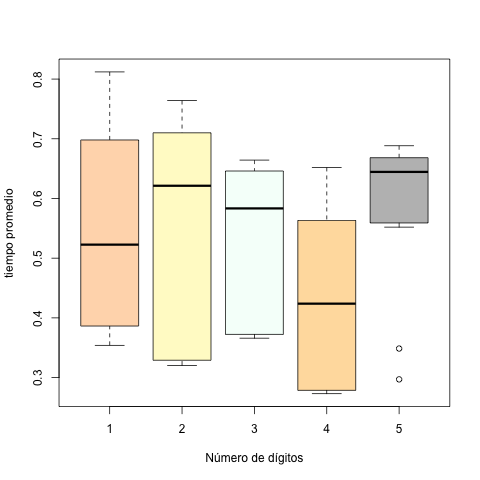
\includegraphics[width=80mm]{./digitos} \label{Dig}}\vspace{-1mm}
\caption{Resultados de ejecución del experimento} \label{Rfin}
\end{figure}


\bibliographystyle{plainnat}

\bibliography{BHWP3}


\end{document} 